\scanpage{73}
\diagram{\begin{tikzcd}
\mathbb Q&\mathbb C\\
H_B^*(X_{\mathbb C})\arrow[r,"\text{oui}",no head]&H_B^*(X)\otimes_{\mathbb Q}\mathbb C
\end{tikzcd}}
\margin{$\mathbb Q$}
\deleted{\uuline{bigradué} \uline{$\unsure{\pi|m.}$}}
\figure{\begin{tikzpicture}
\node[draw,ellipse,align=left] at (0,0) {oui\\\unsure{mais tordu}};
\draw (-1,-.4)--(-.7,.4);
\node[draw,ellipse] at (3,0) {\uuline{non}?};
\draw (2.4,.4)--(2.7,-.4);
\end{tikzpicture}}
\diagram{\begin{tikzcd}[column sep=small]
\unsure{L|K}&\deleted{H_{Hdg}(X)}\arrow[dr,no head]&H_{DR}\arrow[d,no head]&\unsure{L|K}\\
&&H_{\mathrm{cris}}&
\end{tikzcd}}
\diagram{\begin{tikzcd}[column sep=small]
H^{\unsure{r|\nu}}(X,\mathcal O_X)\arrow[r,no head]&H^{\unsure{r-1|\nu-1}}(X,\Omega_X^1)\arrow[r,no head]\arrow[d,no head]&{}\\
&{}\arrow[r,no head]&H_{\mathrm{cris}}
\end{tikzcd}}
\deleted{$\unsure{H^r|H^\nu}(X,\mathcal O_X$}

$i_1$

\deleted{$H_{DR}(X)\otimes_{\mathbb R}\mathbb C\simeq H(X_{\mathbb C},\mathbb R)\otimes_{\mathbb R}\mathbb C$}
\deleted{\diagram{\begin{tikzcd}H_{DR}^*(X_L)\arrow[r,no head]&H_{DR}^{\unsure{*|1}}(X_{\mathbb C})\end{tikzcd}}}
\deleted{$\sigma_1.\sigma_2=f$}
\inserted{\unsure{autom.} \unsure{galois}}
\[
Q^\sigma\simeq Q
\]
\diagram{\begin{tikzcd}X_{\mathbb R}\arrow[r,no head]&X_{\mathbb C}\end{tikzcd}}
\[
H^*(X(\mathbb C),\mathbb C)
\]
\deleted{$H^*(X$}
\[
G
\]
\figure{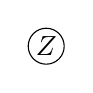
\begin{tikzpicture}\node[draw,circle,inner sep=1pt] {$\unsure{\mathbb Z}$};\end{tikzpicture}}
\[
S\subset\operatorname{Spec}(\mathbb Z)
\]
\deleted{\diagram{\(\begin{array}{c@{\quad}c}
\left\{\begin{array}{c}\boxed{\begin{array}{c}T_B\\T_{DR}\end{array}}\\T_{Hdg}\end{array}\right.&\begin{array}{ll}:&G_B\\:&G_{DR}\\&\end{array}
\end{array}\)}}
\margin{\deleted{\diagram{\begin{tikzcd}\unsure{S}\arrow[d,no head,"\unsure{lisse}"]\\\operatorname{Spec}\mathbb Z\end{tikzcd}}}}
\margin{\figure{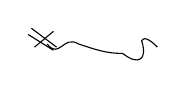
\begin{tikzpicture}[x=.4cm,y=.4cm]
\draw (0,2)--(.8,1.5);\draw (.1,2.2)--(.9,1.6);\draw (.2,1.6)--(.8,2.1);
\draw (.6,1.7) .. controls (1,1.2) and (1.1,2) .. (1.6,1.7) .. controls (2.2,1.5) and (2.5,1.4) .. (3,1.4) .. controls (3.5,1) and (3.8,1.2) .. (3.6,1.8) .. controls (3.7,2) and (4,1.7) .. (4.1,1.6);
\end{tikzpicture}}}

a) $M$ \unsure{module} à conn. intégrable \inserted{sur $S$}, avec \uline{filtration}.

b) \diagram{\begin{tikzcd}M(p)^\sigma\arrow[r,"F_p"]&M(p)\end{tikzcd}} Frobenius \deleted{\unsure{au}} (hom de cristaux)

c) $\mathbf M(\mathbb R)$ fibré \inserted{analytique \deleted{\unsure{filtré}}} (sur $S(\mathbb R)$), muni d'un autom. $F_\infty$ d'ordre $2$.

d) \deleted{$\unsure{B}$} $T$ (betti) système local sur $S_{\mathbb C}^{\deleted{\unsure{*}}\mathrm{an}}$ ($\Rightarrow\pi_1(S_{\mathbb C}^{\mathrm{an}},s)\to\operatorname{Aut}(T_s)$)

e) $T_p$ syst. local sur $S-S_p$ \qquad $T_p\simeq T\otimes_{\mathbb Z}\mathbb Z_p$ sur $S_{\mathbb C}$

$\unsure{f_\infty)}$ $M_{\mathbb C}^{\mathrm{an}}\simeq T\otimes_{\mathbb Z}\mathbb C$

$f_p)$ \qquad $-\ -\ -\ -\ -$
\mspage{72}
